\documentclass[a4paper]{IEEEtran}

\usepackage{graphicx}
\usepackage[numbers,square,comma]{natbib}
\usepackage{hyperref}
\usepackage{eurosym}

\title{Cloud Computing: \\ Report}
\author{Steffan Norberhuis\\ 1509306 \and
 Rogier Slag\\ 1507761}

\author{
    \IEEEauthorblockN{Steffan Norberhuis, Rogier Slag}\\
    \IEEEauthorblockA{1509306, 1507761}
}

\begin{document}
\maketitle
\begin{center}
\today
\end{center}

\section{Abstract}

Over the last few years the web has become a place for multimedia.
With this change, the demand for quick and scalable video conversion has grown.
To make videos available to the largest possible set of consumers, these have to be transcoded to various formats and resolutions.
Meanwhile, this needs to be done at the lowest costs, while the conversion time should not suffer.

This report introduces a prototype of an online, cloud-based, and scalable solution which optimizes for cost, while the conversion time is not significantly affected. 
Additionally, the application can easily cope with random failures of workers.
The final result is described and benchmarked to allow comparisons to other systems.

\section{Introduction}


WantCloud B.V. is the European market leader in fast and cheap video conversion.
Unfortunately, their server systems are quite outdated and therefore expensive to run.
If no action is taken now, they might lose their competitive advantage.

To remain market leader and lower waiting times when there is a high demand, the CEO of WantCloud requested an in-depth investigation of the possibilities to utilize external resources, such as an IaaS-provider (Instrastructure as a Service).
Using the \textit{cloud} for these purposes would have several advantages:

\begin{enumerate}
\item Only pay for the number of machines needed at a time.
\item Flexibility of number of worker nodes (scale up and down quickly)
\item Economy of scale of the IaaS owner for system administrators and hardware.
\item Lower up-front costs and less hardware failures
\end{enumerate}

In this paper the authors propose a solution and present an implementation, complete with benchmarks.
FFmpeg is used to handle the video conversion itself and Amazon Web Services is used as the IaaS-provider.
The software is developed in Java. For provisioning related activity, SSH is employed.

\textit{Proposed solution}: Using the flexibility of EC2, Amazons cloud computing platform, one can continuously run one instance to monitor the number of requested jobs, the cluster status, and notify customers once their jobs completed.
This instance, the master node, therefore performs the roles of \textit{scheduler}, \textit{provisioner}, and \textit{health checker}.
The probability this node goes down is low, and in case it goes down it may easily be restarted on any other node.
More advanced solutions can be developed that will recover from failure of the master node.

Additionally the provisioner can start extra workers, using the API made available by Amazon.
It does this based on parameters which can easily be modified, such as maximum task to worker ratio, max number of workers, or maximum waiting time.
Since the system runs many workers, the likelihood of one failing is much larger. 
Hence in case of a failure the worker should be terminated, removed from the cluster, and its jobs rescheduled.

This paper is structured as follows:
Section 3 will deal with the background of the application.
Section 4 will explore the design of the system and any policies involved. 
Section 5 will show the experimental setup and show and interpret the benchmarks which were run.
In section 6 a discussion is done on the results.
This then leads to a conclusion in section 7.

Any source code discussed in this report and the report itself is available publicly on \href{https://github.com/snorberhuis/CloudComputing}{Github}.

\section{Background on Application}

The application has as goal to convert any user submitted video to an MPEG-4 format (note this format is covered by several patents in countries which acknowledge software algorithms patents \cite{mpegla}.
Users can use the existing client software of WantCloud to upload their video to the servers and receive a notification of the same application once the conversion is done.

In the background, transparent to the user, the video is added to the job list by the scheduler software running on the incoming server.
This scheduler, together with the part which handles provisioning of VM's on an IaaS-provider, places the job on a server for conversion.
Due to the CPU-intensive nature of video-conversion, a server is considered busy if there is one job running on it, and idle if no job is running on it. 
No server will handle two jobs at once.
The provisioner may decide to spin up additional VM's based on several, operator-defined, criteria.
Once the conversion is done, the worker VM uploads the new file to the output server, which then performs a callback on the earlier mentioned client application.

\textit{Requirements:} For the system to work in production, it should ensure the following requirements are met:

\begin{enumerate}
\item For the system to work well for WantCloud B.V., it should have a better performance compared to the existing platform, while at the same time it should have lower monthly operational costs,
\item The system should work completely automated, requiring no intervention for worker nodes. This goes for the autoscaling, handle worker failures, and scheduling.
\item The system should monitor its own state, both in terms of performance as well as for availability.
\item The results should remain available for users to re-download, hence durability is important.
\end{enumerate}


\section{System Design}

\subsection{Resource Management Architecture}

The system is designed using a regular client-server model.
Customers can upload their videos using the application.
The application (not part of this implementation) uploads the video to an Amazon S3 bucket.
This bucket is regularly scanned by the master instance, which generates jobs corresponding to a video and places the jobs into a queue.
The master instance then assigns these jobs to worker nodes, based on a first-come-first-serve principle.
Once a job is done, the result is saved to another Amazon S3 bucket, where the file is available for download.

This approach has multiple advantages.
First of all, all information is durable and the data will be preserved (even in case all instances go down).
Secondly one is able to take down the master instance (e.g. for a new deployment) without affecting the customers ability to upload new videos to the system.
Third, the system achieves the ability for fair multi-tenancy.
Multiple users can at the same time upload a video to the input bucket.
These videos are fairly serviced at a first-come-first-serve principle
and are processed.
Scaling of worker nodes ensures that one users does not influences the delay of another user.

The master instance consists of several components:

\begin{enumerate}
\item
The scheduler:
this part of the application regularly checks for new files and add them to the queue.
The first item in the queue is assigned to the next available worker.
\item
The provisioner:
this section has the responsibility to monitor the number of workers nodes, spawn new ones when thresholds are met, and handles the creation and termination of worker nodes.
\item
A health checker, which is responsible to ensure every node in the cluster is healthy, it requests checks from worker nodes at a regular interval.
Once a worker node fails to respond a certain number of checks, it is considered to have failed and is terminated by the provisioner.
The job of the failed worker node is added to the front of the queue and rescheduled.
\end{enumerate}

All thresholds and settings are managed by a simple configuration file (`scheduler.properties`).
The current system is based on Amazon as a provider, but this implementation can be easily changed to also support other providers such as Microsoft Azure.

For simplicity the system has one job list, to which each new job is added.
Each job keeps track of its status which can be one of the following: `QUEUED`, `STARTED`, `FINISHED`, or `FAILED`.
Jobs are downloaded from and uploaded to AWS S3 using the AWS SDK, which offers a TransferManager abstraction layer to handle the IO operations to the workers nodes.
The videos remain in the input bucket and this allows the system to reschedule a job if a worker node fails.

Workers nodes are provisioned using the same SDK and are started by executing a simple script through SSH.
A worker will then get its source directly from Github, build the Maven project and start running.
By responding to the health checks, the provisioner is made aware that the start proces has been completed and the node is added to the pool. 
The scheduler will now start assigning jobs to the node.
If a node fails to come online within five minutes, a failure is assumed and the node is terminated again.

The worker nodes contain as little logic as possible and this makes them to be ready for termination at any moment.
Each node is required to communicate with the master instance.
Messages are sent for each assignment (from master to worker), each status update (from worker to master) and for health checks (bidirectional).
Since all information is gathered at the master instance, this is also the location where statistics regarding performance are stored.

To improve reliability, the assumption is made that a worker node can fail at any given point in time
and the system has to be prepared for this.
To adequately build the system to handle this, a system called \textit{Chaosmonkey} was introduced.
Chaosmonkey can be configured to run at a certain interval and with a certain probability.
In the case that Chaosmonkey does run it will pick a worker node 
and simulate a complete node failure.
The Chaosmonkey communicates directly with Amazon, so neither the worker nor the master instance know what happened and should simply react to the results of the health check.
However, it will log its activity to the master instance log, such that an operator can easily see whether a failure was intended.
The Chaosmonkey makes failure a natural part of the system performance.
This forces one to always deal with failure and tests reliability.
Chaosmonkey is an idea that was published and is used by Netflix in their production environment \cite{Netflix-cm}.

\subsection{System Policies}

The system always uses a elastic scaling policy. There are several parameters which can be set to define the policy.

\begin{enumerate}
\item A task should not be waiting for over a certain number of seconds.
If that is the case, under-capacity is anticipated and new nodes are provisioned.
\item The ratio between tasks and nodes should not exceed a set threshold. 
If that is the case, it is assumed that there is too little capacity, so a new node is provisioned.
\item While a new node is being provisioned, no other provisioning will start.
\item A maximum number of nodes can be specified to avoid very high costs by a DDoS similar attack.
\end{enumerate}

As one can see the provisioning scheme is fairly conservative.
There are several good reasons for this.
First from talks at WantCloud it was discovered an incidental delay is not problematic.
Secondly many \textit{eager} provisioning schemes in the cloud suffer from oscillation, where a set of nodes is constantly being created and terminated.
In the time between their creation and termination, they can only complete a few jobs.
The provisioning time outweighs the production time and hence are a waste of resources and money).
Hence in this case the decision was made to focus on cost-efficiency over performance.

Once a VM goes idle and there is no new job for it to process, it will be terminated.
This termination policy is no problem for the node creation policy: since no new node will be started immediately, but the system waits for a node to become free (or at some point will start a new node). 
This solves the oscillation problem for the system.

\section{Experimental Results}
In this section the experimental setup and the experiments themselves are described.
Observations and experiments are also included in this section.

\subsection{Experimental setup}

The system was developed for Amazon AWS and was tested on that platform.
Amazon AWS provides different types of instances, for this case the \emph{t2.medium} instances were used.
This type was chosen because it is most likely the type that will be used by WantCloud B.V..
The type has a good balance between performance and cost for the specific type of application used by WantCloud B.V..
Video conversion itself is mostly CPU intensive, so the instances with 2.5GHz and 1 GB of memory could be outperformed by larger instances or compute optimised instances.

A specially designed workload generator creates a new task at a regular interval and offers this task to the system using the input bucket.
The task can either be a completely new task or, with a certain chance, be a task earlier offered to the system.
The tasks consist of encoding a movie from one format to another format.
The workload generator introduce quite rapidly a high number of tasks for the system
and can be seen as a large number of users using the system at the same time.
But without extra information of WantCloud B.V. this cannot be put into perspective.

To monitor the system \emph{The Simple Logging Facade for Java} (SLF4J) in combination with \emph{Log4J} were used, which allowed optimal and tunable logging.
SLF4J provides a facade for Log4J to allow other logging backends to be configured at runtime.
For this specific case simple logging output was employed to measure the performance and other statistics of the system.
%other tools

\subsection{Experiments}

\subsubsection{Automation}
No specific experiments were ran to test the automation of the proposed system, but the other experiments have shown that a very high level of automation was been achieved.
To start only a handful of mandatory steps had to be done, after which the system runs completely without manual intervention.
The first step is to create a EC2 instance which will act as a master instance.
After that one uploads the code and runs an install script that sets up the master instance.
The last step is to build the code and run it.
This sequence takes around one minute once the instance is accessible by SSH.

\subsubsection{Elasticity}

The first experiment aimed to answer how long it takes to provision a worker node and how long it takes before it is fully ready to service tasks.
The experiment consists of the provisioner provisioning continuously a single worker after the previous worker has become fully ready.
The experiment showed that the average and median time of provisioning a fully working node is 2 minutes and 31 seconds.
The minimum time of provisioning was 2 minutes and the maximum 4 minutes and 47 seconds.
A note has to be made that the timing is done with a granularity of 15 seconds, because that was the interval at which the health check was performed.
The results are therefore somewhat longer than the moment the instances were actually ready.
But this experiment still gives a very good indication of the time it takes to provision a worker node.

The second experiment conducted was to let the workload generator generate 100 jobs with a random delay of 10 to 30 seconds between jobs.
The experiment is to test that the provisioner provisions more nodes and terminates these nodes after these 100 jobs are completed.
At first the system builds a backlog of jobs and the provisioner conservatively allocates more workers.
After 27 minutes all jobs are finished and it can be seen that the provisioner quickly terminates the now unnecessary workers.
While downscaling, a very eager approach is used which helps to optimize for cost.
At the end a tail can be seen where one worker is kept running.
This data is plotted in Fig. \ref{fig:100-workers} and Fig. \ref{fig:100-tasks}.

Here a cost indication of the running costs of the system is given.
This is done by calculating the cost of running the previous experiment.
The total time the experiment took was 36 minutes.
But during this time several machines were used.
In total the machines were hired for the equivalent of hiring one machine for 31 hours.
Using the calculation model of Amazon the charged time would be 31 hours and the charged cost would be \euro 3,40.


\begin{figure}[ht]
	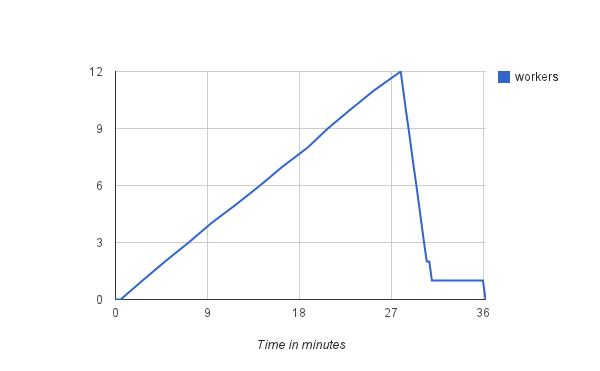
\includegraphics[scale=0.45]{fig/100workers.png}
	\label{fig:100-workers}
	\caption{Amount of workers}
\end{figure}

\begin{figure}[ht]
	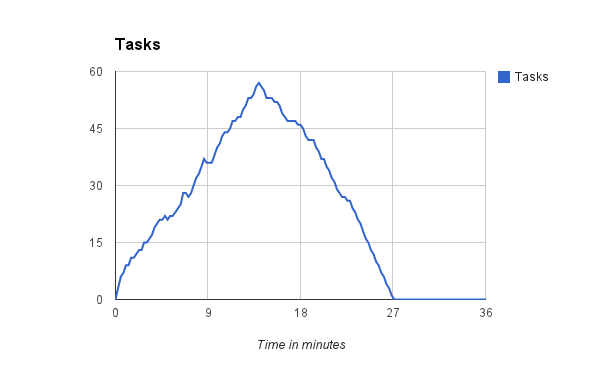
\includegraphics[scale=0.45]{fig/100tasks.png}
	\label{fig:100-tasks}
	\caption{Amount of queued tasks}
\end{figure}

\subsubsection{Performance}
Load balancing is very important to achieve a higher utilization of the VMs.
Early during the development of the proposed system CPU utilization of the used VMs was measured.
It was found that FFmpeg is very effective and used the full CPU power during execution.
As there is no more performance to be gained, scheduling more tasks on a single node could not achieve a higher utilization.
This was the main reason to let one node only work on one job at once.

\subsubsection{Reliability}
To test reliability, Chaosmonkey was activated during a similar experiment conducted to test the elasticity with a workload of 100 jobs.
The Chaosmonkey performs a run every 4 minutes with a chance of 50\% to let a node fail.
The results can be seen in Fig. \ref{fig:chaos-workers}.
Here small drops can be seen and at that moments Chaosmonkey terminated a worker node.
The system detects failure and reschedules the tasks and continues with the jobs.
Afterwards the granularity of the amount of workers was improved to see the effects of the Chaosmonkey.
This changes the appearance of the figure from Fig. \ref{fig:100-workers}.

\begin{figure}[ht]
	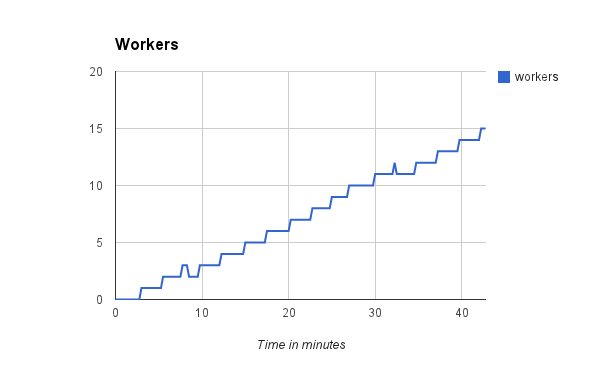
\includegraphics[scale=0.45]{fig/chaos-workers.png}
	\label{fig:chaos-workers}
	\caption{Amount of workers with Chaos monkey activated}
\end{figure}

\subsubsection{Monitoring components}
No specific experiments were conducted to test the monitoring components.
But they were used extensively to conduct the other experiments and take measurements.

\section{Discussion}
The developed system has proven that the application of WantCloud B.V. can be transfered to the Cloud with relative ease.
This is largely due to the good API and simplicity of using instances provided by Amazon AWS.
So the development time and cost should not be a reason for WantCloud B.V. for not choosing to use a cloud platform.
The system can still be improved on multiple areas,
but it is a very respectable result for the total development time that was put into it.

Failure within cloud platforms are notorious and has to be taken into account during development.
But the system has shown that reliability and fault recovery can easily be introduced
and even be a natural part of the system.
Again, this is not a reason for WantCloud B.V. to not move to the cloud.

Performance is not thorougly tested enough through our experiments that a conclusive decision can be made based upon this criteria.
On one hand do the worker node achieve high CPU utilization, but on the other hand do the experiment show a continuous build up of tasks.
This might partially be the provisioning not being aggressive enough in provisioning nodes.
But could also be a hint that the instances produce not enough performance to handle the workload.
To really make a decision based upon this criteria more experiments have to be run
where both a non cloud solution and a cloud solution receive the same, realistic workload.
The realistic workload can also help produce an accurate estimation of costs as will later be explained not to be possible at the moment.

For development and experimentation the Amazon AWS system was used and during that time numerous instances were used.
Long experiments were conducted, not all reflected in the paper, that took several hours to complete.
At some point we let the master instance continuously run during several nights, so we did not have to provision it every time and install the software.
The choice was made to not use the cheapest instances, but higher tiered instances.
As they were believed to be more realistic choices.
This only resulted in a total cost of \$ 5.61 for 437 charged hours.
Noteworthy is that the costs of storage was only \$0.18.
This is remarkable,
 because we used large files and uploaded multiples of these files.
The rest of the costs is for the instances.

The workload generator simulates multiple users at the same time.
But without any real information of usage patterns estimating for 100,000/1,000,000/10,000,000 users would be total guess work.
The calculation of costs per day/month/year depends on the amount of users and required instances and the distribution of size of videos.
Again this calculation would result in total guess work because it depends on realistic usage information.

The deletion schedule currently optimizes costs with the assumption that lower costs can be achieved when the ratio between provisioning time and production time is minimized. 
But the schedule can result in a situation where high costs are incurred,
because the scheduler never runs out of tasks and worker nodes are kept indefinitely alive.
As was said before some delay is acceptable and lower costs could perhaps be achieved if more worker nodes were terminated at the cost of a higher delay.
This should be investigated in future experiments.

\section{Conclusion}

In this report, a elastic cloud based system was proposed to handle different kinds of video conversion.
Consequently, the performance and costs were analyzed for a representative test set using Amazon Web Services as an IaaS provider.
From the results in the experimental section one can see that the provisioning is done conservatively, whereas the termination of nodes is done eagerly.
This provides a nice optimization for costs.

On the other hand, once a node has been provisioned it will continue to perform jobs until there is no more work for it. 
This will allow the system to fully utilize the node in order to minimize the non-production time (the time between one started paying for the computing power and the moment the node could start its first job).
This timespan is mostly dependent on the cloud provider and the method of provisioning.
Using very simple software on the nodes, the installation of the node can be done in around one minute.
Another minute is needed to actually \textit{lease} the machine from the provider, in this case Amazon.
\bibliography{bibliography}
\bibliographystyle{unsrtnat}
\appendix
\section{Time Sheets}
\end{document}
